\documentclass[tikz,border=5pt]{standalone}
\usepackage{tikz}
\usetikzlibrary{arrows.meta}
\definecolor{nebula}{HTML}{6366F1}
\definecolor{spark}{HTML}{14B8A6}
\definecolor{ink}{HTML}{334155}
\begin{document}
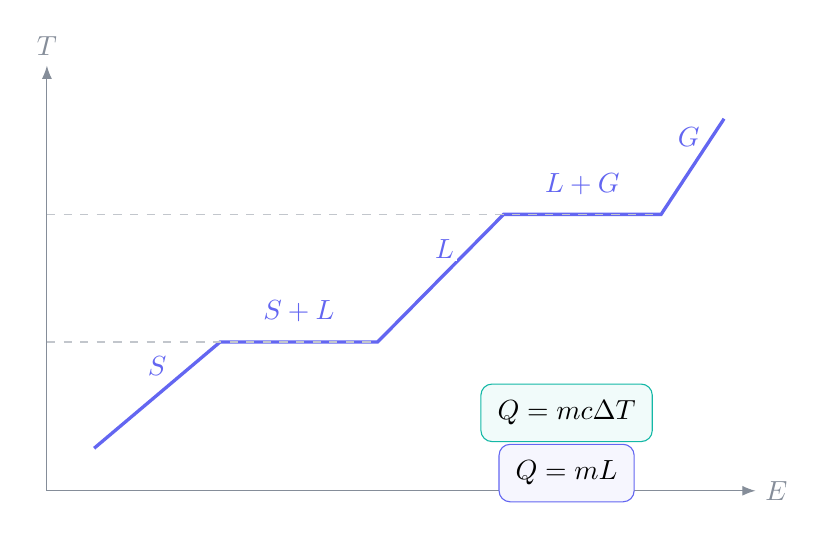
\begin{tikzpicture}[x=1cm,y=.9cm,font=\sffamily,>=Latex]
  \draw[->,ink!60] (0,0)--(9,0) node[right] {$E$};
  \draw[->,ink!60] (0,0)--(0,6) node[above] {$T$};
  \draw[very thick,nebula] (.6,.6)--(2.2,2.1)--(4.2,2.1)--(5.8,3.9)--(7.8,3.9)--(8.6,5.25);
  \draw[dashed,ink!30] (0,2.1)--(4.2,2.1);
  \draw[dashed,ink!30] (0,3.9)--(7.8,3.9);
  \node[nebula,above=6pt,sloped,fill=white,inner sep=1pt] at (1.4,1.35) {$S$};
  \node[nebula,above=6pt,fill=white,inner sep=1pt] at (3.2,2.1) {$S+L$};
  \node[nebula,above=6pt,sloped,fill=white,inner sep=1pt] at (5.05,3.0) {$L$};
  \node[nebula,above=6pt,fill=white,inner sep=1pt] at (6.8,3.9) {$L+G$};
  \node[nebula,above=6pt,sloped,fill=white,inner sep=1pt] at (8.15,4.58) {$G$};
  \node[draw=spark,rounded corners=4pt,fill=spark!6,inner sep=6pt] at (6.6,1.1) {$Q=mc\Delta T$};
  \node[draw=nebula,rounded corners=4pt,fill=nebula!6,inner sep=6pt] at (6.6,.25) {$Q=mL$};
\end{tikzpicture}
\end{document}
